	\section{Modeling for global verification}
	
	
	
	\subsection{Classical encoding}
	
    The most straightforward idea to encode the global verification question is to 
    consider variable $x_j,\hat{x}_j$ and $x'_j,\hat{x}'_j$ for nodes of the image $I$ and of its perturbation $I'$,
    using the classical encoding (\ref{eq11}) for each variable, that we call $\mathcal{M}^{classical}$.
    
    use two identical MILP models, one for 
    , i.e., to build a model  
    
    based on two identical MILP models $\mathcal{M},\mathcal{M}'$ with completely disjoint variables (and their own constraints) plus some extra constraints:
	\begin{enumerate}
		\item Add constraints for connecting input nodes $\mathcal{M},\mathcal{M}'$ to meet the requirement $|\boldsymbol{x}-\boldsymbol{y}| \leq \varepsilon$.
		\item Set the optimization objective as the difference between two variables of the same output node in two models $\mathcal{M},\mathcal{M}'$ (because we want to compute $\max|f(\boldsymbol{x}) -f(\boldsymbol{y}) |$).
	\end{enumerate}
	This large model contains twice as many binary variables as $\mathcal{M}$. The computational cost of solving an MILP model grows roughly exponentially with the number of binary variables, and hence it will cost much more time.
	
	We may relax some constraints (by changing binary variables to continuous variables) as in the case of local robustness. However, the problem is that even relaxing a few nodes can cause a significant loss of accuracy, which motivates us to explore other modeling approaches.
	
	\subsection{A Simplified model}
	
	To avoid above problem, we introduce a simplified model that is to use one variable $y_i$ to represent the difference of each two variables: that is, if $x_i$ and $x'_i$ are two variables in $\mathcal{M}$ and $\mathcal{M}'$ representing the same node, then we set $y_i=x_i-x'_i$ and and $\hat{y}_i=\hat{x}_i-\hat{x}_i'$. The relation between $y_i$, $x'_i$ and $\hat{y}_i$ is $\hat{y}_i = \ReLU(x'_i+y_i)-\ReLU(x'_i).$ 
	
	Given  $\gamma_i$ be the upper bound of $y_i$, the constraints for $\hat{y}_i$ are the follows:\begin{align*}
		\hat{y}_i &\leq a \gamma_i               &\quad \hat{y}_i &\geq y_i - a \gamma_i \\
		\hat{y}_i &\geq (a-1) \gamma_i           &\quad \hat{y}_i &\leq y_i + (1-a) \gamma_i
	\end{align*} where $a$ is a binary variable.
	
	
	The following plot illustrates the constraints described above.
	
	\begin{figure}[b!]
		\centering
	\hspace*{10ex}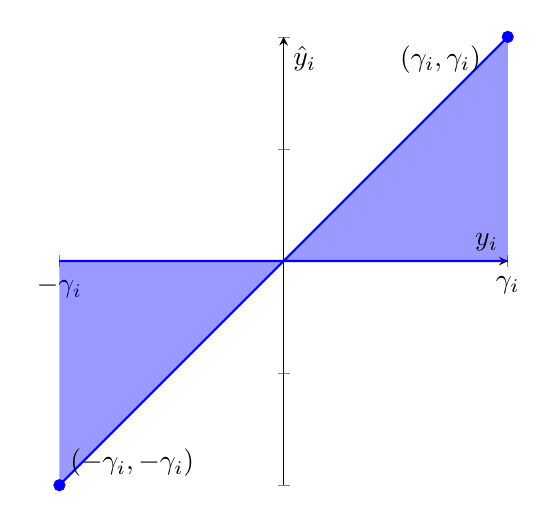
\begin{tikzpicture}
		\begin{axis}[
			xlabel={$y_i$},
			ylabel={$\hat{y}_i$},
			xmin=-2, xmax=2,
			ymin=-2, ymax=2,
			axis lines=center,
			samples=100, 
			unit vector ratio=1 1 1, scale=1, xtick   = {-2,2},
			xticklabels = {$-\gamma_i$,$\gamma_i$},
			yticklabels = {},
			]
			\addplot[blue, thick, fill=blue, fill opacity=0.4] {x} \closedcycle; 
			\addplot[blue, thick] {0}; 
			
			\addplot[only marks, mark=*, mark size=2pt, blue] coordinates {(-2,-2)};
			\node[label={above:$(-\gamma_i,-\gamma_i)$}] at (axis cs: -1.35, -2.1) {};
			
			\addplot[only marks, mark=*, mark size=2pt, blue] coordinates {(2,2)};
			\node[label={above:$(\gamma_i,\gamma_i)$}] at (axis cs: 1.4, 1.5) {};
		\end{axis}
	\end{tikzpicture}
\caption{The possible values of $\val(\hat{y}_i)=\ReLU(\val(x_i))-\ReLU(\val(x'_i))$ depending on $\val(y_i) = \val(x_i)-\val(x'_i)$.}
	\label{fig.1v}
\end{figure}


	
	Based on above constraints, we can sketch this simplified model:
	\begin{enumerate}
		\item For each input node, each output node, and each pre-activation and post-activation node in the hidden layers,  set one variable $y_i$. 
		\item Set constraints for input nodes.
		\item Set linear constraints . In this case, since the meaning of $y_i$ is $x_i-x'_i$, this constraints will not use the bias.
		\item Between pre- and post- activation nodes, set the MILP constraint described above.
	\end{enumerate}
	
	The key point is that, although this model sets 3 variables (and their binary variables) for each node in the network, only $y_i$  contributes to the final results, and we can ignore $x_i,x_i'$ (and their binary variables) during the optimization.
	
	As a result, we can relax the binary variables used to $\hat{x}_i = \ReLU(x_i)$ and $\hat{x}'_i = \ReLU(x'_i)$.
	
	Now the simplified model contains the same number of binary variables as the MILP model for local robustness. Hence this model runs much faster compared to the previous one. The trade-off is lower accuracy compared to the first model under unlimited time. In practice, with a reasonable timeout, this simplified model can usually obtain a better bound.
	
	One major disadvantage of this model is that the solution obtained through optimization may not be valid-i.e., the output computed by the network on the optimized inputs may not equal the output value in the solution. Nevertheless, it is meaningful to compute the upper bound. 
	
	%	However, in practice, with a reasonable timeout, this simplified model can usually obtain a better bound.
	%	
	\subsection{Improving the Accuracy of the Simplified Model}
	We can remove the disadvantage and improve the accuracy of the above simplified model by modifying the constraints, at the cost of increased computational time — a trade-off between accuracy and speed. 
	
	%	(This model has the same binary set, although the meaning of binary variable for $y_i$ is somehow different.)
	
	
	
	%	The exact constraints for $$ \begin{align*}
		%		&\hat{y}_i \geq -\hat{x}'_i \hspace*{1ex} \wedge \hspace*{1ex} \hat{y}_i \leq -\hat{x}'_i+a\beta_i  \hspace*{1ex}\wedge\hspace*{1ex} x_i'+y_i \leq a\beta_i \hspace*{1ex}\wedge\hspace*{1ex}  x_i'+y_i \geq (1-a)\alpha_i \\
		%		&\hat{y}_i \geq -\hat{x}'_i+(x_i'+y_i) \hspace*{1ex}\wedge\hspace*{1ex} \hat{y}_i \leq -\hat{x}'_i+(x_i'+y_i) +(a-1)\alpha_i \\
		%	\end{align*} 
	%	
	%	
	%	Moreover, we can add two more natural constraints: $x_i'+y_i \geq \alpha_i \hspace*{1ex}\wedge\hspace*{1ex}  x_i'+y_i \leq \beta_i.$
	
	
	
	
	
	\begin{figure}[t!]
		\centering
	\hspace*{-10ex}
	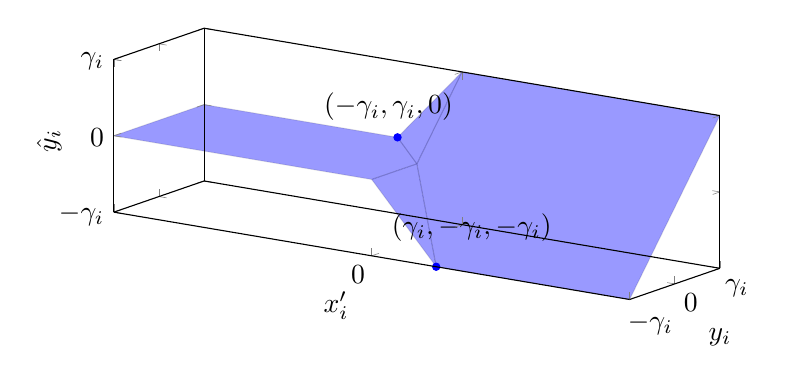
\begin{tikzpicture}[scale=0.65]
		\begin{axis}[	axis on top, xlabel = \(x'_i\),
			ylabel = {\(y_i\)}, zlabel = \(\hat{y}_i\),
			set layers=default,
			xmax = 4, xmin = -4,
			ymax = 1, ymin = -1,		
			zmax = 1, zmin = -1,
			unit vector ratio=1 1 1, scale=2.5,  ytick   = {-1,0,1},
			yticklabels = {$-\gamma_i$,$0$,$\gamma_i$}, xtick = {0},
			xticklabels = {$0$}, ztick   = {-1,0,1},
			zticklabels = {$-\gamma_i$,$0$,$\gamma_i$},
			view={35}{14},
			]
			\addplot3[ fill=blue,opacity=0.1, fill opacity=0.4] 
			coordinates {
				(0,0,0) (-1,1,0) (-4,1,0) (-4,-1,0) (0,-1,0) (0,0,0)
			};
			
			\addplot3[	fill=blue,opacity=0.1, fill opacity=0.4] 
			coordinates { (0,0,0) (0,1,1) (4, 1, 1) (4, -1, -1) (1,-1,-1) (0,0,0)
			};
			
			\addplot3[	fill=blue,opacity=0.1, fill opacity=0.4	] 
			coordinates { (0,0,0)  (-1,1,0) (0,1,1) (0,0,0)
			};
			
			\addplot3[	fill=blue,opacity=0.1, fill opacity=0.4	] 
			coordinates { (0,0,0)  (0,-1,0) (1,-1,-1) (0,0,0)
			};
			
			\addplot3[only marks, mark=*, mark size=2pt, blue] coordinates {(1,-1,-1)};
			\node[label={$(\gamma_i,-\gamma_i, -\gamma_i)$}] at (axis cs: 1.2, -0.5 ,-1) {};
			
			\addplot3[only marks, mark=*, mark size=2pt, blue] coordinates {(-1,1,0)};
			\node[label={$(-\gamma_i,\gamma_i, 0)$}] at (axis cs: -1, 0.8 ,0) {};			
		\end{axis}
	\end{tikzpicture}
	\caption{The outcome $\val(\hat{y}_i)=\ReLU(\val(x_i))-\ReLU(\val(x'_i))$ 
	depending on $\val(y_i) = \val(x_i)-\val(x'_i)$ and on $\val(x'_i)$.}
	\label{fig.2v}
\end{figure}
	
Given $\gamma_i$ as the upper bound of $y_i$, $\alpha_i,\beta_i$ be the upper and lower bound of $x_i,x_i'$, 
	the precise  constraints for $\hat{y}_i = \ReLU(x'_i+y_i)-\ReLU(x'_i)$ (along with $\hat{x}'_i=\ReLU(x'_i)$) are as follows:
	\begin{align*}
		& \begin{aligned}
			y_i + x'_i &\leq a\beta_i        &
			y_i &+ x'_i \geq (1-a)\alpha_i \\
			x'_i       &\leq a'\beta_i       & 
			x'_i       &\geq (1-a')\alpha_i \\
			\hat{y}_i  &\leq a\gamma_i       &
			\hat{y}_i  &\geq -a'\gamma_i \\
			\hat{y}_i  &\leq y_i + (1-a)\gamma_i  &
			\hat{y}_i  &\geq y_i - (1-a')\gamma_i \\
			\hat{y}_i  &\leq -x'_i + a\beta_i &
			\hat{y}_i  &\geq -x'_i + (1-a')\alpha_i \\
			\hat{y}_i  &\leq y_i + x'_i + (1-a)(-\alpha_i) &
			\hat{y}_i  &\geq y_i + x'_i + a'(-\beta_i)
		\end{aligned}
	\end{align*} Here, $a,a'$ are binary variables, and $a'$ is also the binary variable in the constraints for $\hat{x}'_i=\ReLU(x'_i)$. 
	

Similar to the second model, the constraints on $x_i$ for $\hat{x}_i=\ReLU(x_i)$ are not necessary, or at least can be relaxed without any loss in accuracy.
	
	%	\begin{align*}
		%		& y_i+x'_i \leq a\beta_i \quad\wedge \quad y_i+x'_i\geq (1-a)\alpha_i\\	
		%		& x_i' \leq a'\beta_i \quad\wedge \quad x_i'\geq (1-a')\alpha_i\\
		%		&\hat{y}_i \leq a\gamma_i \quad\wedge \quad	\hat{y}_i \geq -a'\gamma_i \\
		%		&	\hat{y}_i \leq y_i+(1-a)\gamma_i \quad\wedge \quad	\hat{y}_i \geq y_i - (1-a')\gamma_i \\
		%		&	\hat{y}_i \leq -x'_i+a\beta_i \quad\wedge \quad	\hat{y}_i \geq -x'_i+(1-a')\alpha_i \\
		%		&	\hat{y}_i \leq y_i+x'_i+(1-a)(-\alpha_i)\quad\wedge \quad	\hat{y}_i \geq y_i+x'_i+a'(-\beta_i) \\
		%	\end{align*} 
	
	The following plot illustrates the constraints described above.
	

	In practice, when we relax the constraints for a node, we will convert $a_i$ and $a_i'$ to continuous variables together. In principle, we can also choose to change  only one of those two binary variables.
	
	%	The relaxation of this model is similar: let $a$s and $a'$s be continuous variables instead of binary/integer variables. Unlike the first model in this section, relaxing a few nodes does not lose too much accuracy.
	
	A special relaxation approach of this model is to treat the binary variables $a'$ appearing in the above constraints and the binary variables for $\hat{x}'_i=\ReLU(x'_i)$ as distinct variables, and relax only the latter. 
	
	This approach has a similar disadvantage as the model in the previous section: the output computed by the network on the optimized inputs may not equal the output value in the solution. Similarly, it is meaningful to compute the upper bound using this approach. 
	